\chapter{The Futhark \csharp{} backend}
In this chapter we first demonstrate how we want to use Futhark-generated
\csharp{} GPU libraries in \csharp{} programs. We then describe the architecture
needed for compiling such \csharp{} libraries using the Futhark compiler, and
what features we need in our code generator to successfully generate standalone
\csharp{} programs embedded Futhark-generated GPU kernels. 
We then show the finished design of the generated Futhark \csharp{} code, and
describe the segments in the code segment by segment.

We discuss choices taken for memory management in Futhark \csharp{} programs,
and compare different methods of memory management by their runtime performance.

Finally, we discuss how and why the OpenCL library ``\texttt{Cloo}'' was chosen
as a backend for Futhark's \csharp{} compiler.

\section{Recap on using Futhark \csharp{} libraries}
For a given Futhark program (such as the one shown in figure \ref{fig:shortfutharkprogram3'}), 
we want to be able to compile the program to a
\csharp{} library from the command line like shown in figure \ref{fig:shortfutharkprogram4'}.
This results in a compiled \csharp{} dynamically linked library\footnote{A
  \texttt{.dll} file}.
Then, we can include this library in a \csharp{} project like any other external
library, and use its functions as expected, like shown in figure \ref{fig:shortfutharkprogram5'}.

\begin{figure}[H]
\begin{subfigure}
  \centering
  \begin{lstlisting}[language=Futhark]
entry mapPlus2 (xs : []i32) : []i32 =
  map (+2) xs
  \end{lstlisting}
  \caption{A short Futhark program called mapPlus2.fut}
  \label{fig:shortfutharkprogram3'}
\end{subfigure}

\begin{subfigure}
  \centering
  \begin{lstlisting}[language=sh]
$ futhark-cs --library -o MapPlus2.dll mapPlus2.fut
  \end{lstlisting}
  \caption{We call the Futhark-to-\csharp{} compiler \texttt{futhark-cs} on
    mapPlus2.fut}
  \label{fig:shortfutharkprogram4'}
\end{subfigure}

\begin{subfigure}
  \centering
\begin{minted}[linenos]{csharp}
using System.Linq;
using MapPlus2;

public class Program
{
    public static int Main(string[] args)
    {
        var mapplus2Class = new MapPlus2();
        var xs = Enumerable.Range(0, 1000000).ToArray();
        var xs_result = mapplus2Class.mapPlus2(xs)
    }
}
\end{minted}
  \caption{We use the compiled Futhark program as any other library.}
  \label{fig:shortfutharkprogram5'}
\end{subfigure}
\end{figure}

\subsection{Compiling and using Futhark \csharp{} executables}
\label{subsec:futharkcsexe}
Not all users are interested in using Futhark programs as parts in other code
projects. Instead, these users can opt to compile Futhark programs into
executables. Recalling the Futhark example in
\Cref{fig:shortfutharkprogram3',fig:shortfutharkprogram4',fig:shortfutharkprogram5'},
we instead opt to compile the Futhark program as an executable program.

Keeping the Futhark source file \texttt{mapPlus2.fut} from
\ref{fig:shortfutharkprogram3'}, we use futhark-cs to compile the program into
an executable; the command line is shown below: %in figure \ref{fig:shortfutharkprogram4''}.
  \begin{lstlisting}[language=sh]
$ futhark-cs -o MapPlus2 mapPlus2.fut
  \end{lstlisting}
%
Here, the compiler produces an executable named \texttt{MapPlus2} from the
original source file, named {\tt mapPlus2.fut}.

We can now execute this program in one of two ways.
The first way is to write our arguments in a string in the command line, and
to \texttt{echo} them through a pipe into the executable, as shown below:
  \begin{lstlisting}[language=sh]
$ echo "[1,2,3,4,5,6,7]" | ./MapPlus2
[3i32, 4i32, 5i32, 6i32, 7i32, 8i32, 9i32]
  \end{lstlisting}
%This method is shown in figure \ref{fig:shortfutharkprogram5''}. 
Here, the one argument we are using is 
an integer array. We pass the array to the executable, and it prints the result
to \texttt{stdout} after it has finished. The \texttt{i32}'s tells us that the
result array holds 32 bit signed integers.
For multi-argument entry functions, we separate the arguments with whitespace.

For the second method, we store our arguments in a dataset file. For example, we
can store our integer array in a plain text file, named {\tt array.in}, 
as shown below: %shown in figure \ref{fig:array.in}.
  \begin{lstlisting}
[1,2,3,4,5,6,7]
  \end{lstlisting}
We can then use the command line to redirect the contents of the dataset file
into our command:
%as shown in figure \ref{fig:shortfutharkprogram5'''}.
  \begin{lstlisting}[language=sh]
$ ./MapPlus2 < array.in
[3i32, 4i32, 5i32, 6i32, 7i32, 8i32, 9i32]
  \end{lstlisting}
If we want to, we can redirect the output from stdout to a file of our own
choice: %shown in figure \ref{fig:shortfutharkprogram6'}. 
  \begin{lstlisting}[language=sh]
$ ./MapPlus2 < array.in > result.txt
$ cat result.txt
[3i32, 4i32, 5i32, 6i32, 7i32, 8i32, 9i32]
  \end{lstlisting}
Here, we redirect Futhark's output to \texttt{result.txt}, and print it to 
\texttt{stdout} by using \texttt{cat} to confirm that we have obtained indeed 
the correct result.

\clearpage

\section{The Futhark \csharp{} compiler architecture}
In figure \ref{fig:ccompiler} we showed a rough sketch of the
Futhark compiler's architecture. To sufficiently explore the contribution of
this thesis, we will however first need a more detailed view of the architecture
we need to implement to accomplish our goal.
This architecture is depicted in figure \ref{fig:futharkcompilerlowerlevel}.

\begin{figure}[H]
  \centering
  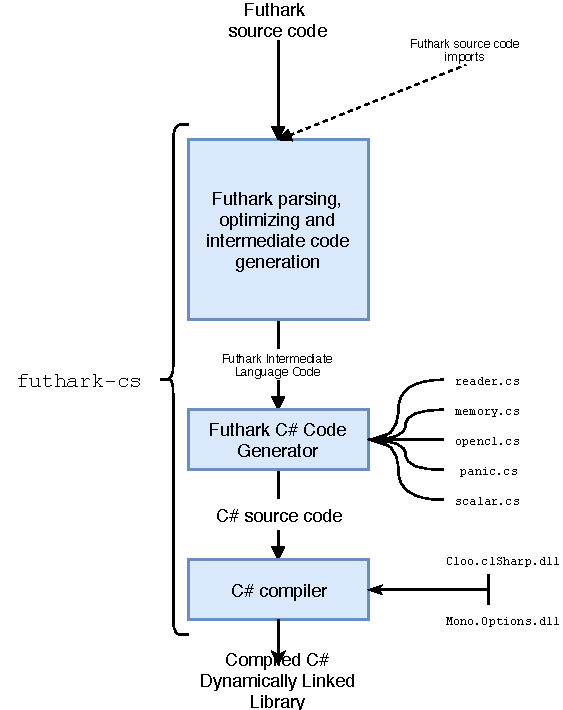
\includegraphics[scale=0.85]{chapters/figs/csharp/futharkcsarchitecture.pdf}
  \caption{The Futhark \csharp{} architecture, including necessary imports.}
  \label{fig:futharkcompilerlowerlevel}
\end{figure}

We will now describe its three main steps:
\begin{description}
\item[Step 1:]\hfill\\
  A Futhark source file is passed to the Futhark compiler (like in figure
  \ref{fig:shortfutharkprogram4'}). Although only the main source file is passed
  as an argument to the compiler, the compiler also includes any imports in the
  main source file, if there should be any.

  This first part of the Futhark compiler is responsible for parsing the passed
  Futhark program, including imports, and performs all type checks, SOAC
  optimizations, fusions and so on~\cite{pldi17}. The result of this process is a
  Futhark program expressed in imperative internal intermediate called \texttt{ImpCode}.
  The \texttt{ImpCode} grammar is included in the appendix. The \texttt{ImpCode}
  language contains everything from memory operations like allocating and
  deallocation memory (both on system memory and on the GPU), interfacing with
  the OpenCL device (like copying buffers back and forth between the system and
  the GPU, setting kernel arguments and launching computation kernels), and also
  basic expressions like addition and multiplication.

\item[Step 2:]\hfill\\
  The \csharp{} code generator takes the Futhark program written in
  \texttt{ImpCode}, and expresses it as \csharp{} source code.
  For example, we can take the simple \texttt{ImpCode} expression in figure \ref{fig:impcode},
  and rewrite it as \csharp{} code, shown in figure \ref{fig:impcodeascs}.
  \begin{figure}[H]
    \centering
\begin{minted}{lisp}
SetScalar "x" (
    BinOpExp Add 
      (ValueExp (IntValue (Int32Value 4))) 
      (ValueExp (IntValue (Int32Value 5)))
    )
\end{minted}
    \caption{Setting int x to 4+5 with simplified \texttt{ImpCode}}
    \label{fig:impcode}
  \end{figure}

\begin{figure}[H]
\centering
\begin{minted}{csharp}
int x = 4 + 5;
\end{minted}
\caption{Setting int x to 4+5 in \csharp{}}
\label{fig:impcodeascs}
  \end{figure}

Besides taking an \texttt{ImpCode} program as input, it also embeds a set of
prewritten \csharp{} libraries\footnote{\texttt{reader.cs} et al} into the generated \csharp{} code. These
libraries are ncessary for the finished \csharp{} program, and are described in
section~\ref{subsec:runtimelibs}.\\
The resulted \csharp{} source code is passed to a \csharp{} compiler, but also
written to disk so it is available for the developer.

\item[Step 3:]\hfill\\
  To use the \csharp{} code, we need to compile it using the command shown in
  figure \ref{fig:callcsc}. We tell the compiler that we have external libraries
  stored at the location stored at \texttt{\$MONO\_PATH}\footnote{An environment
  variable that should be set to a directory containing external runtime
  libraries for Mono runtime usage.}, and we tell the compiler to
  reference two extra external libraries \texttt{Mono.Options.dll} and
  \texttt{Cloo.clSharp.dll}, as we need these libraries in the Futhark \csharp{} programs.

  We also add the library flag ({\tt -lib}) so that \texttt{csc} compiles to a \texttt{.dll} file instead of
  generating an executable. Finally we add the \texttt{/unsafe} flag so the
  compiler allows us to use \texttt{unsafe} statements in the \csharp{} program.

\begin{figure}[H]
  \centering
  \begin{lstlisting}[language=sh]
$ csc -lib:$MONO_PATH -r:Mono.Options.dll \
      -r:Cloo.clSharp.dll /unsafe mapPlus2.cs
  \end{lstlisting}
  \caption{Calling the \csharp{} compiler on the resulted {\tt mapPlus2.cs} file.}
  \label{fig:callcsc}
\end{figure}

However, the last step in \texttt{futhark-cs} does this for the user
automatically, as long as the user has set the required \texttt{\$MONO\_PATH}
variable, and that the directory that \texttt{\$MONO\_PATH} points to, contains the
required libraries.

\end{description}

This thesis leverages the already existent Futhark codebase to implement 
steps 1 and 3, hence does not bring important contributions to them. 
Instead, the contribution of this thesis refers to implementing the 
code generator described in step 2.

%\subsection{Designing the Futhark \csharp{} generator}
In the grand scheme of things, the Futhark \csharp{} generator is not
interesting by itself. The entire contribution to the Futhark compiler is
around 4500 SLOC, split 50/50 between \csharp{} and Haskell code.
In the remaining of this chapter we will instead discuss at a high level
the {\em structure of the generated code}.

%\clearpage

\section{The Structure of the Generated \csharp{} Code}
As previously discussed, Futhark code can be compiled (1) to a library 
that is usable in both \csharp{} and \fsharp{} programs, and (2) also
to a standalone \csharp{} executable, which, for example, takes argument 
inputs from the \texttt{stdin} stream, and prints the
results to \texttt{stdout}.

As this thesis focuses on interoperability, we will primarily concentrate on the
design of the \csharp{} code generated for Futhark libraries, and mention
design differences in the cases in which the Futhark executables differs 
from the translation used for libraries.
Figure \ref{fig:futharkcsclasses} shows a high level representation of the
generated \csharp{} classes for the standalone- and library-compilation cases.

\begin{figure}[h]
  \centering
  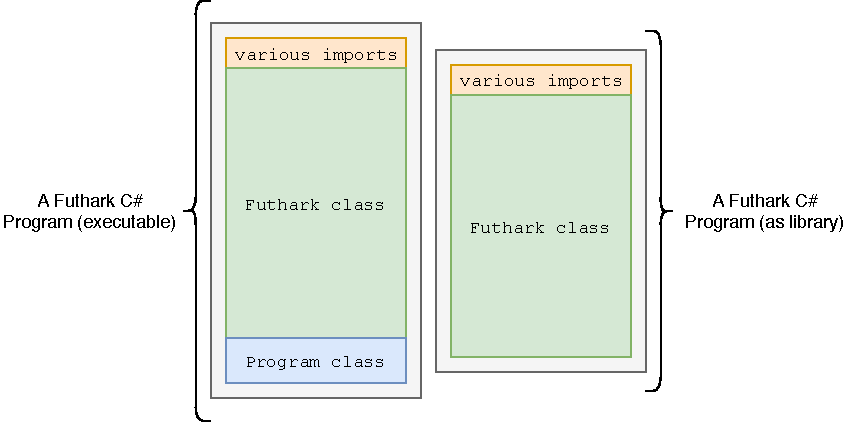
\includegraphics[scale=0.85]{chapters/figs/csharp/futharkcs_wide.pdf}
  \caption{The two possible types Futhark \csharp{} programs}
  \label{fig:futharkcsclasses}
\end{figure}

Here follows a short explanation of the different sections of the Futhark
programs.
\begin{description}
\item[\texttt{various imports}] \hfill \\
  This part consists of \texttt{using} statements that import the
    various libraries on which the translation relies into the \csharp{} program.
  
\item[\texttt{Futhark class}] \hfill \\
  The Futhark class is a singleton class that encapsulates all needed functionality
    for executing the exports (entry-points) defined in the original Futhark file.
  The Futhark class is discussed in subsec \ref{subsec:futharkclass}.
  
\item[\texttt{Entry functions}] \hfill \\
  The entry functions wrappers for the exports declared in the Futhark program,
    that are mainly responsible for converting the human-readable input into
    the internal (``machine'') representation expected by the export implementation.
  For example an array can be passed string, but needs to be translated to
  a one dimensional array of bytes.

\item[\texttt{Program class}] \hfill \\
  In the case of Futhark libraries, the entire \csharp{} program consists
  of the imports and the Futhark class. Only for executables do we add the entry
  functions to the Futhark class, and the Program class to the \csharp{} source
  file itself.
 
  The Program class contains a Main method, which is necessary for the \csharp{}
  program to be compiled as an executable. This design is discussed in \ref{subsec:programclass}
\end{description}

\subsection{The Futhark class design}
\label{subsec:futharkclass}
The Futhark class is the single class defined in the compiled Futhark library.
It is depicted in figure \ref{fig:futharkclass}. 
The following subsections explains the various parts of the class.
\begin{figure}[h]
  \centering
  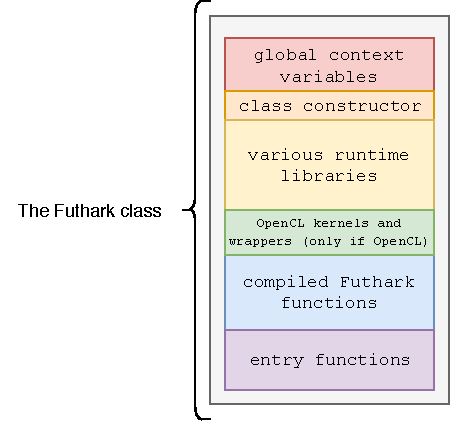
\includegraphics{chapters/figs/csharp/futhark_class.pdf}
  \caption{An overview of the Futhark class}
  \label{fig:futharkclass}
\end{figure}


\subsubsection{Global context variables}
\label{globalcontextvariables}
Compiled Futhark programs need to keep track of several variables.
Both normal and OpenCL-enabled Futhark \csharp{} programs can take several
options when they're launched from the command line. In example,
\texttt{num\_runs} tells the Futhark runtime how many times the chosen entry
function should be executed, and the variable \texttt{runtime\_file} tells the
Futhark runtime where it should write timing information to, for example for
benchmarking purposes.

Instead of passing an argument array along throughout all the functions in the
Futhark class, like we usually would do if we were writing purely functional
programs, we instead represent these arguments as class variables, which 
are set when the class is instantiated. 
This allows to refer to them from wherever in the rest of the class
(without passing them explicitly as arguments).

For non-OpenCL programs, these variables are exclusively used for benchmarking and
debugging purposes. For OpenCL programs however, the global variables are vital
for the program's execution.
In an OpenCL program, the Futhark class must keep track of two extra
variables.

The first variable is \texttt{struct futhark\_context ctx} and contains 
the global state of the current program's execution. The global state consists of 
\begin{itemize}
    \item[(1)] the current list of unused but allocated OpenCL buffers on the device, 
    \item[(2)] kernel handles for all the OpenCL kernels used in the Futhark program,
    \item[(3)] a counter for the total running time of the program.
    \item[(4)] the  \texttt{opencl\_context}, which holds the metadata necessary for
                OpenCL execution, for example the current state of the device, 
                the queue of in-execution OpenCL actions, and so forth.
\end{itemize}

The second variable is \texttt{struct futhark\_context\_config cfg} and records
configuration information necessary for constructing the actual 
\texttt{futhark\_context}.

\subsubsection{The class constructor}
The class constructor is necessary to setup the global variables needed
throughout the Futhark class. When the Futhark program is compiled as an
executable, the command line arguments are passed to the class constructor by
the \texttt{Program} class. If the Futhark program is compiled as a library, the
programmer can pass a string array of arguments to this constructor manually.

Besides setting class variables, OpenCL-enabled versions will initialize (and
set) first the \texttt{futhark\_context\_config cfg} variable, and afterwards
the \texttt{futhark\_context} itself.

\subsubsection{The various runtime libraries}
\label{subsec:runtimelibs}

The runtime libraries are a set of seperate \csharp{} files that are written and
distributed through the Futhark compiler. When a Futhark program is compiled,
these library files are concatenated and embedded directly into the rest of the
generated code. They contain functionality which the generated Futhark programs
depend on.
The runtime libraries are the following:
\begin{description}
\item[\texttt{memory.cs}] \hfill\\
  Futhark's imperative IR ({\tt ImpCode}) represents all arrays---no matter of 
    their dimensionality and primitive-element type---as a flat one-dimensional 
    array of bytes, which are accompanied by an array of 64-bits integers 
    recording the dimensions of the flat array.  As such it was necessary to 
    define a set of functions that are able to interact with these byte arrays,
    e.g., if the original array was holding {\tt float}s, than we need to be
    able to read/write a float value from/into the byte array. 
  For example, \texttt{memory.cs} contains the \texttt{writeScalarArray} functions,
  which writes a scalar value to a certain location into the byte array. The 
    function is overloaded so it works with scalars of any integer or floating 
    point primitive types. Figure~\ref{fig:writeScalarArray} shows the instance
    of {\tt writeScalarArray} that writes a value of type {\tt double} into the
    byte array.
\begin{figure}[h]
\centering
\begin{minted}[fontsize=\small]{csharp}
void writeScalarArray(byte[] dest, int offset, double value)
{
    unsafe
    {
        fixed (byte* dest_ptr = &dest[offset])
        {
            *(double*) dest_ptr = value;
        }
    }
}
\end{minted}
\caption{\texttt{writeScalarArray} writes a value at the specified offset in
some byte array.}
\label{fig:writeScalarArray}
\end{figure}

\item[\texttt{scalar.cs}] \hfill\\
  This library contains all the scalar functions necessary for Futhark \csharp{}
  programs.
  In Futhark, arithmetic operators are defined for integers and floats of all
  sizes, and bitwise operators are defined for all integers.
  However, this is not the case in \csharp{}, where many arithmetic operators
  are only defined for 32- and 64 bit integers.
  
  If these operators are used with 8- or 16 bit operands, the operands are
  implicitly casted to 32 bit integers at compile time, which also means that
  the final result of the operation is a 32 bit integer, which doesn't has the
  right type.

  Therefore, wrapper functions must be defined for even the simplest arithmetic
  functions. For example, integer addition in \csharp{} Futhark is actually
    implemented by four different functions:
\begin{minted}[fontsize=\small]{csharp}
static sbyte add8(sbyte x, sbyte y){ return Convert.ToSByte(x + y); }
static short add16(short x, short y){ return Convert.ToInt16(x + y); }
static int add32(int x, int y){ return x + y; }
static long add64(long x, long y){ return x + y; }
\end{minted}

  Besides, \texttt{scalar.cs} also contains the \csharp{} definitions for the various
  mathematical functions from Futhark's \texttt{math.fut}library, such as \texttt{exp},
  \texttt{sin} and \texttt{cos}.


\item[\texttt{reader.cs}] \hfill\\
  The reader contains the entire functionality for recieving function parameters
  through \texttt{stdin}, as shown in the example in subsec
  \ref{subsec:futharkcsexe}.
  The reader reads scalars of any of the Futhark-supported primitives, and also arrays and multidimensional arrays of scalars.

  The reader also supports reading streams of binary data. This enables Futhark
  to parse datasets that are stored as pure byte representation, instead of
  string representations.
  It is only necessary for Futhark executables.
  

\item[\texttt{opencl.cs}] \hfill\\
  \texttt{opencl.cs} contains wrapper functions for \texttt{OpenCL}'s memory
  related functions. In example, instead of calling \texttt{clCreateBuffer} directly for
  allocating an \texttt{OpenCL} buffer, we call \texttt{OpenCLAlloc} from
  \texttt{opencl.cs}. By using a wrapper function instead of calling
  \texttt{clCreateBuffer}, we encapsulate functionality and employ better error
  handling.
  The wrapper functions in \texttt{opencl.cs} also employs a \texttt{free list} for \texttt{OpenCL}
  memory allocations. This list is stored in the \texttt{futhark\_context}, and
  has the following functionality:
  \\
  1) When the Futhark program frees an \texttt{OpenCL} buffer, it is not
  actually freed, but is instead added to the \texttt{free list}.\\
  2) When the Futhark program later allocates an \texttt{OpenCL} buffer, it
  first goes through the \texttt{free list} to see, whether it can use one of the already
  existing allocations instead.
\end{description}

\subsubsection{The compiled Futhark functions}
  The compiled Futhark functions are the Futhark functions as written in
  \texttt{ImpCode}\footnote{See figure \ref{fig:impcode}}, expressed in the
  target language, in this case \csharp{}.

  The compiled Futhark functions corresponds to the entry functions found
  in the entry functions-section of the Futhark class.
  Only the Futhark \texttt{entry} functions are compiled to individual functions, and
  remaining helper functions are inlined here.

  In OpenCL programs, all array functions and SOAC calls are compiled as
  individual (or fused) OpenCL kernels. Therefore, the compiled Futhark
  functions in these programs consists of mainly some scalar operations and
  memory allocations, and calls to Futhark-generated kernel wrapper functions.
  There are also mixes, in example \texttt{for-}loops that call OpenCL kernels.
  
  In non-OpenCL programs, the array functions and SOAC calls are not stored in
  seperate wrapper functions, but inlined in the Futhark functions.

\subsubsection{OpenCL kernels and wrappers}
  If the Futhark program is compiled for OpenCL, all array handling function- and
  SOAC calls are compiled as OpenCL kernels. This part of the Futhark class
  has two parts:
  \begin{enumerate}
  \item The string (actually a single string in an array) \texttt{opencl\_prog}, which contains the entire
  Futhark-generated OpenCL source code for the Futhark program in question.
  This source code contains all the OpenCL kernels for the program, and is
  passed to the OpenCL device, compiled and loaded, when the Futhark class is
  initialized. Handles to the individual kernels are then stored in the \texttt{futhark\_context}.

  \item For each kernel in the \texttt{opencl\_prog}, the Futhark compiler
    generates a kernel wrapper function. These wrapper functions takes the
    kernel arguments (such as scalar values, array values and indexes) as input,
    and performs all the OpenCL specific work necessary for the actual kernel
    launch; in example setting the kernel arguments on the device, and copying
    data back and forth between host and device buffers.
  \end{enumerate}

\subsection{Entry functions}
\label{csharpentries}
Futhark's internal representation of array values are one dimensional byte
arrays (which can represent arrays of any type and dimensionality), and an
accompanying list of integers denoting the lengths of the array's dimensions.
However, Futhark does not expect it's users to pass this form of arrays as
function arguments, which is why each Futhark \texttt{entry} function has a
corresponding entry function in the final compiled code.
\\\\
To discern between Futhark functions and entry functions, the Futhark function's
name is prefixed with ``\texttt{futhark\_}'', as in for example
``\texttt{futhark\_foo}''.
Depending on whether the Futhark program is compiled as an executable or a
library, the entry function itself is then named ``\texttt{entry\_foo}'' or
just ``\texttt{foo}''.

For executables, ``\texttt{entry\_foo}'' is a function that doesn't take any
arguments. Instead, it uses the reader functions from \texttt{reader.cs} to parse the
arguments for ``\texttt{foo}'' from \texttt{stdin}, and passes them to the
Futhark function. For all array values in the arguments, the array values are
converted into Futhark representations of them.
When the Futhark function returns the result, the result is then printed to \texttt{stdout}.

\subsection{Entry functions in executables}
\label{entryfunctionsinexecutables}
Consider again our small Futhark program mapPlus2 (figure \ref{fig:mapplus20}).
\begin{figure}[H]
  \centering
  \begin{lstlisting}[language=Futhark]
entry main (xs : []i32) : []i32 =
  map (+2) xs
  \end{lstlisting}
  \caption{A short Futhark program called mapPlus2.fut}
  \label{fig:mapplus20}
\end{figure}

If we compile this program as an executable, we get Futhark/entry function pair
shown in figure \ref{fig:futharkentrypairexe}. The example is very simplified
but does resembles the actual implementation in functionality.

By calling \texttt{entry\_main()}, we first call \texttt{ReadStrArray<int>} to parse an integers
array from stdin. We then read the number of elements in the array into a
variable, and then convert the integer array to a byte array, as Futhark
functions use byte arrays for internal value array representation.

We then call the internal Futhark function, which returns a byte array, the
length of the byte array and the number of elements that the byte array
represents.
We reform the byte array into an integer array, and print the result to \texttt{stdout}.

\begin{figure}[H]
  \centering
\begin{minted}[linenos, breaklines]{csharp}
(int, byte[], int) futhark_main(int byte_array_length, byte[] byte_array, int byte_array_elms)
{

    // ...
    // futhark stuff happens
    // ...

    return (out_array_length, out_array, out_array_elms);
}

void entry_main()
{
    var (int_array, lengths) = ReadStrArray<int>(1, "i32");
    var int_array_elms = lengths[0];
    var byte_array = convertToByteArray<int>(int_array);
    var byte_array_length = byte_array.Length;

    var (res_array_memsize, res_array, res_array_elms) =
        futhark_entry(byte_array_length, byte_array, int_array_elms);

    var res_array_as_ints = reform_array<int>(res_array, res_array_elms);
    printArray(res_array_as_ints);
    exit(0);
\end{minted}
  \caption{A simplified Futhark/entry function pair from the mapPlus2 executable}
  \label{fig:futharkentrypairexe}
\end{figure}

\subsection{Entry functions in libraries}
If we compile the program in fig \ref{fig:mapplus20} program as a library, we get Futhark/entry function pair
shown in figure \ref{fig:futharkentrypairlib}. The example is very simplified
but does resembles the actual implementation in functionality.

The difference between this example and the example in 
section~\ref{entryfunctionsinexecutables} is that the arguments of the Futhark export
are passed directly to the wrapper (e.g., {\tt entry\_main}) instead of being parsed
from {\tt stdin}. Similarly, the result of the wrapper is the type-casted result of
the Futhark export as opposed to the result being written to \texttt{stdout}.
\begin{figure}[H]
  \centering
\begin{minted}[linenos, breaklines]{csharp}
    (int, byte[], int) futhark_main(int byte_array_length, byte[] byte_array, int byte_array_elms)
    {

        // ...
        // futhark stuff happens
        // ...

        return (out_array_length, out_array, out_array_elms);
    }

    (int[], int[]) entry_main(int[] int_array, int[] int_array_lengths)
    {
        var int_array_elms = int_array_lengths[0];
        var byte_array = convertToByteArray<int>(int_array);
        var byte_array_length = byte_array.Length;

        var (res_array_memsize, res_array, res_array_elms) =
            futhark_entry(byte_array_length, byte_array, int_array_elms);

        var res_array_as_ints = reform_array<int>(res_array, res_array_elms);
        var res_lengths = new int[] { res_array_as_ints.Length };
        return (res_array_as_ints, res_lengths);
\end{minted}
  \caption{A simplified Futhark/entry function pair from the mapPlus2 library}
  \label{fig:futharkentrypairlib}
\end{figure}

\subsection{Type signature for entry functions}
\label{subsec:flatarraysinentryfuncs}
Currently, library functions aren't callable with jagged arrays (arrays of 
pointers to arrays), but must instead be called with a flat element array,
which is paired up with an array of lengths denoting the dimensionality of 
the flat element array. This is explained in sec \ref{aaaa}.

The \fshark{} implementation offers helper functions that can flatten jagged
arrays into flat arrays/dimension array pairs, and back again.
In the future, this might be added to the Futhark \csharp{} backend for
usability purposes.

\clearpage

\subsection{The Program class design}
\label{subsec:programclass}
As shown in figure \ref{fig:futharkcsclasses}, we only add the Program class to
the Futhark program so we have an entrypoint for the executable.
The entire Program class is depicted in figure \ref{fig:programclass}, with the
contained source code and all.

\begin{figure}[H]
  \centering
  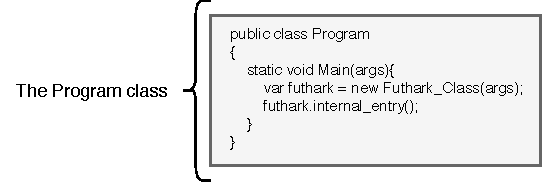
\includegraphics{chapters/figs/csharp/program_class.pdf}
  \caption{The complete functionality of the Program class for Futhark
    executables.}
  \label{fig:programclass}
\end{figure}

%%% \section*{The \csharp{} backend, compared to the C- and Python counterparts}
%%% 
%%% %% DESCRIBE THE DIFFERENCES BETWEEN C# AND THE REST
%%% THE PYTHON BACKEND HAS MUCH FUNCTIONALITY ENCAPSULATED IN PYOPENCL, AND DOESN'T
%%% NEED TO DECLARE VARIABLES BEFORE SETTING THEM
%%% LESS COMPLEX GENERATOR NEEDED AS VARIOUS OPENCL STATEMENTS ARE HANDLED
%%% AUTOMATICALLY BY LIBRARY
%%% 
%%% C BACKEND MUST BE AWARE OF ALL SIZES AND EVERYTHING AT COMPILE TIME, WHICH MEANS
%%% STATES MUST BE ALLOCATED THROUGH COMPLEX STRUCTS AT COMPILE TIME, AND STRUCTS
%%% MUST BE DEFINED AT COMPILE TIME AS WELL
%%% 
%%% C ALLOWS NULL POINTERS, CS DOES NOT WHICH MEANS WE NEED PLACEHOLDER VARIABLES
%%% 
%%% CSHARP GENERATOR IS SOMEWHERE INBETWEEN AS IT IS CAN HANDLE OBJECTS WHICH CAN
%%% CARRY STATE, FURTHERMORE DYNAMIC MEMORY ALLOCATION
%%% 
% THE DIFFERENCES BETWEEN MEMORY HANDLING IN CS AND CSOPENCL
\section{Memory management in Futhark \csharp{}}
As Futhark stores array values in byte arrays, it is relevant to compare
the difference between how the array handling differs between Futhark's C
backend, and this \csharp{} backend.
For OpenCL programs, the memory management of \csharp{} and C is largely the
same, as the OpenCL side of these programs are the same. \csharp{} does after
all just use C bindings for it's OpenCL interactions.

However, for non-OpenCL \csharp{} programs, we have to take \csharp{}'s memory
model into consideration.

C implicitly allows unsafe programming. In this case, it means interacting with system
memory by reading and writing arbitrary values from/to arbitrary locations,
designating the values and destinations as whatever type we want.
In figure \ref{fig:futharkcscene}, we see a \texttt{for}-loop that
performs a prefix-sum operation on an array of integers.
On line 6, reading from right to left, we are first creating a reference to
a location in the byte array \texttt{xs\_mem\_4223}. However, as the reference
is a pointer to a byte in the array, we must recast it as an \texttt{int32\_t} pointer.
After we do this, we can finally dereference the pointer to retrieve a four byte
integer from the byte array.

We add the retrieved integer to our accumulating variable
\texttt{scanacc\_4187}, before we cast a reference in our destination byte array
as an integer pointer, and store the result there.

\begin{figure}
\centering
\begin{minted}[linenos, fontsize=\small]{c}
memblock mem_4226;
memblock_alloc(&mem_4226, bytes_4224);
int32_t scanacc_4187 = 0;

for (int32_t i_4189 = 0; i_4189 < sizze_4135; i_4189++) {
    int32_t x_4147 = *(int32_t *) &xs_mem_4223[i_4189 * 4];
    
    scanacc_4187 += x_4147;

    *(int32_t *) &mem_4226[i_4189 * 4] = scanacc_4187;
}
\end{minted}
\caption{A short snippet from a Futhark C program}
\label{fig:futharkcscene}
\end{figure} 

In \csharp{}, arrays and lists are accessed by indexing, i.e. \texttt{var
  x = myArray[10];}.
These arrays are managed by .NET's CLR\footnote{Common Language Runtime}, and
access violations, such as indexing out of bounds, makes the CLR raise a suitable
exception, which can be handled in the \csharp{} program by catching it
accordingly.

However, for performance reasons\ref{marshalunsafeperformance}, we are 
interested in writing to our \csharp{} arrays directly.
To do this, we must use both \texttt{unsafe} blocks and \texttt{fixed} blocks.
Note that this does not necessarily result in unsafe code, because the Futhark
generated code is performing the safety checks already.

\subsubsection{The \texttt{unsafe} block}
In \csharp{}, we cannot just write arbitrary values to arbitrary locations, as this
opens the program for memory access violations by trying to access memory
outside of \csharp{}s memory space. Such violations triggers segmentation faults
which halts the entire program, instead of throwing an exception.

Therefore we encapsulate our unsafe pointer-using code in an \texttt{unsafe}
block.

\subsubsection{The \texttt{fixed} block}
\csharp{}s CLR manages memory locations for allocated buffers, which means that
it also moves these memory allocations around in memory during program execution
when necessary.
To be able to read and write to buffers referenced by pointers, we must
therefore fix these buffers in memory, before we are able to use them directly.

An example of using the unsafe- and the fixed block is shown in figure
\ref{fig:writeScalarArray'}. We start the function by starting an
\texttt{unsafe} block. After we have started the \texttt{unsafe} block, we fix
the destination buffer in memory and get a pointer to the exact location that we
are interested in. Finally, we use a cast to treat the destination pointer as a
\texttt{double} pointer so we can store a \texttt{double} at that location.
\begin{figure}[h]
\centering
\begin{minted}[fontsize=\small]{csharp}
void writeScalarArray(byte[] dest, int offset, double value)
{
    unsafe
    {
        fixed (byte* dest_ptr = &dest[offset])
        {
            *(double*) dest_ptr = value;
        }
    }
}
\end{minted}
\caption{\texttt{writeScalarArray} writes a value at the specified offset in
some byte array.}
\label{fig:writeScalarArray'}
\end{figure}

\subsection{Performance}
\label{marshalunsafeperformance}
Although \csharp{} does offer safe methods to store values directly in byte
arrays, we have chosen to avoid these functions as their implementations carry
huge overhead compared to doing things the unsafe way.
For this benchmark, we are writing N integers to a byte array, using the three
methods shown in figure \ref{fig:threemethods}.
\begin{figure}
  \centering
  \begin{minted}{csharp}
static void UsingBuffer()
{
    byte[] target = new byte[TEST_SIZE*sizeof(int)];
    for (int i = 0; i < TEST_SIZE; i++)
    {
        var intAsBytes = BitConverter.GetBytes(i);
        Buffer.BlockCopy(intAsBytes, 0, target, i * sizeof(int), sizeof(int)); 
    }
}

static void UsingUnsafe1()
{
    byte[] target = new byte[TEST_SIZE*sizeof(int)];
    for (int i = 0; i < TEST_SIZE; i++)
    {
        unsafe
        {
            fixed (byte* ptr = &target[i * sizeof(int)])
            {
                *(int*) ptr = i;
            }
        }
    }
}

static void UsingUnsafe2()
{
    byte[] target = new byte[TEST_SIZE*sizeof(int)];
    unsafe
    {
        fixed (byte* ptr = &target[0])
        {
            for (int i = 0; i < TEST_SIZE; i++)
            {
                *(int*) (ptr+i*sizeof(int)) = i;
            }
        }
    }
}

\end{minted}
  \caption{Three methods of writing integers to an array.}
  \label{fig:threemethods}
\end{figure}


The full program is available in listing \ref{fig:memoryperformancebenchmark} in the
appendix, to compare safe and unsafe methods of writing values to byte arrays, and the
results (as shown in fig \ref{fig:shortperformancegraph}) tells us that there
are definite performance gains to retreive by going \texttt{unsafe}.

The obvious reason for the performance difference is, that for the safe
method, in each of the N iterations, the BitConverter allocates a small 
array of bytes, where the value of integer-scalar {\tt i} is recorded,
and then it copies this small array into the target byte array. 
The unsafe methods do not exhibit this overhead, since they update directly
the target byte array. 
The performance difference between the second and third method corresponds to
the small overhead that comes from fixing the target buffer in memory.

\begin{figure}
    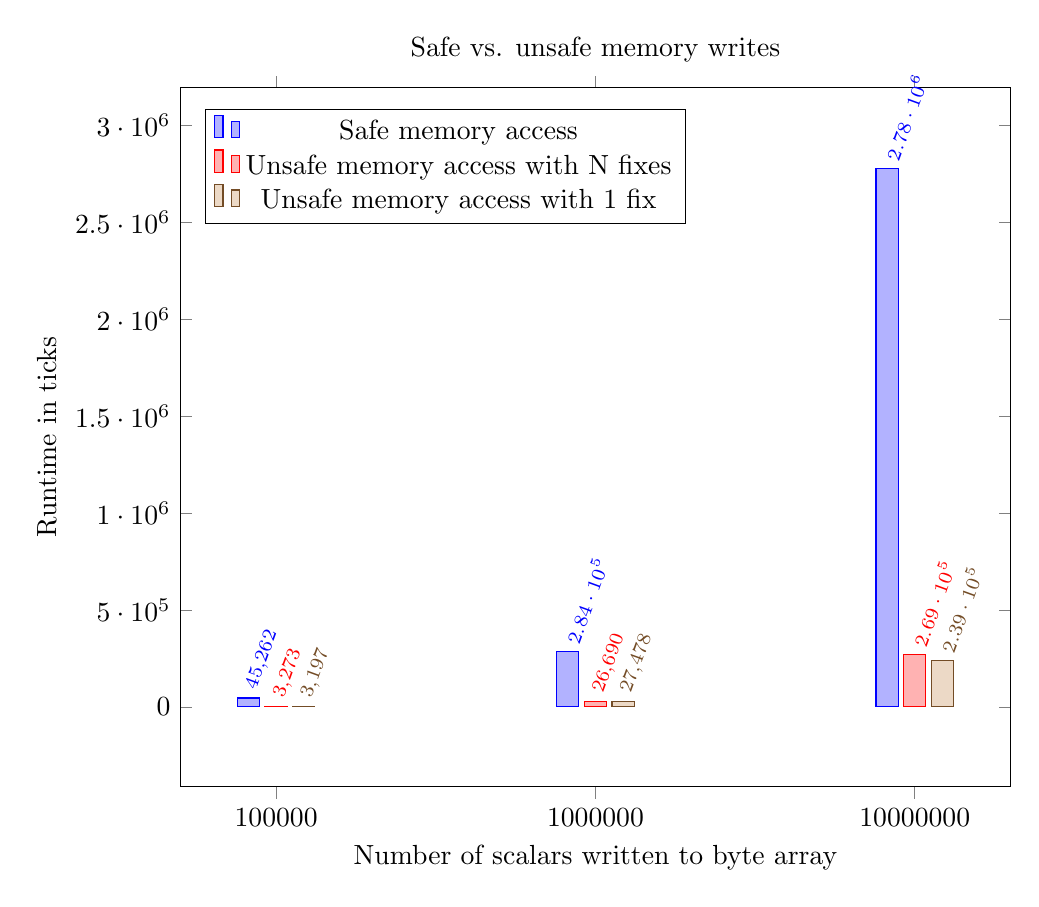
\begin{tikzpicture}
      \begin{axis}[
        title={Safe vs. unsafe memory writes},
        xlabel={Number of scalars written to byte array},
        ylabel={Runtime in ticks},
        width=1\textwidth,
        %height=0.5,
        scaled y ticks=false,
        symbolic x coords={100000, 1000000, 10000000},
        xtick=data,
        enlargelimits=0.15,
        ybar=2pt,% configures ‘bar shift’
        bar width=8pt,
        nodes near coords,
        every node near coord/.append style={rotate=70, anchor=west,font=\scriptsize},
        legend style={legend pos=north west}
      ]
      \addplot plot coordinates {(100000, 45262 ) (1000000, 284379) (10000000, 2778424)};
      \addplot plot coordinates {(100000, 3273 ) (1000000, 26690) (10000000, 268978)};
      \addplot plot coordinates {(100000, 3197 ) (1000000, 27478) (10000000, 238691)};
      \legend{Safe memory access, Unsafe memory access with N fixes, Unsafe memory access with 1 fix}
      \end{axis}
    \end{tikzpicture}
    \caption{Comparison between safe and unsafe methods for writing scalars in a byte array.}
    \label{fig:shortperformancegraph}
\end{figure}

\section{Selecting an OpenCL interface for \csharp{}}
OpenCL interaction is not a part of the .NET standard library, but several
libraries do exist for .NET/OpenCL interactions. For this thesis, I researched a
selection of these libraries, to determine which one that would fit the best for
my purposes.
As Futhark depends on being able to interface with the OpenCL platform directly,
it was necessary to find an OpenCL library for .NET which had direct bindings to
the OpenCL developer library.

The .NET libraries I took into consideration was \texttt{NOpenCL}, \texttt{OpenCL.NET} and \texttt{Cloo}.
All three libraries have been designed to aide OpenCL usage in \csharp{}
programs, by simplifying OpenCL calls behind abstractions, in example by
wrapping pointer operations in private methods.
\\
\\

\begin{description}
\item[\texttt{NOpenCL}]\hfill\\
\texttt{NOpenCL} was the first candidate for the \csharp{} backend, and had
several advantages to the other two: As per February 2018, it had been updated
within the last year, and was therefore the least deprecated library. Second,
the \texttt{NOpenCL} repository on Github contains both unit tests and
example programs.

However, \texttt{NOpenCL} is also tailored for Windows use, and therefore not a
good fit for Futhark, as Futhark is available on both Windows, Linux and Mac OS.
Furthermore, the library is not available through the NuGet
package manager, and the OpenCL API calls are needlessly complex to work with
through the library.

\item[\texttt{OpenCL.NET}]\hfill\\
\texttt{OpenCL.NET} also has a test suite, is available through NuGet, and is
used as the backend for other libraries, such as the \fsharp{} GPU library
\texttt{Brahma.FSharp}.

However, this library hardcoded to work on a in a Windows context, and has not been
updated for more than five years.

\item[\texttt{Cloo}]\hfill\\
\texttt{Cloo} is usable on all three
platforms, and it is available on NuGet. Furthermore, as opposed to the other two libraries, the
Cloo library contains a class with static functions that does nothing but
passing arguments on to the OpenCL library, using \csharp{}s \texttt{DllImport}
attribute. It is immediately possible to skip most of \texttt{Cloo}s features,
and just use the library for it's OpenCL bindings.

Furthermore, the \texttt{Cloo} project is still alive, and the \texttt{Cloo}
\texttt{develop} branch on Github is actively being updated as per July 2018\footnote{\url{https://github.com/clSharp/Cloo/commits/develop/Cloo/Source}}.
\\
\\
\end{description}
Given these three candidates, I chose to work with \texttt{Cloo}: It was the
only one that had the necessary OpenCL bindings readily available, and the only
one that was platform agnostic.
%%% Local Variables:
%%% mode: latex
%%% TeX-master: "../thesis"
%%% End:
